\chapter{Neural Network}

An artificial neural network network mimics the working of a real brain. The brain exists of neurons that transmit information via synapseses. The computer science way to mimic these neurons is shown in figure \ref{fig:nnd}. These work in the bigger context as shown in figure \ref{fig:nno}. In this figure you see different kinds of layers, the input layer (which handles the input), the hidden layer(s) (which pass information) and the output layer (the results). To go from one layer to next you weight the input data, and pass it through the function in the neuron. The function in the neuron is a threshold function (aka activiation function). It is basically the sum of all of the weighted values above or below a certain value. If it is above the threshold the neuron fires a signal (1) otherwise it fires (0). This in turn is then weighted and passed to the next neuron untill the output layer is reached. To optimise we can actually drop the threshhold value (thanks to Paul Werbos) and use a sigmoid function instead for making the decisions. The weights are initially chosen at random and will be optimised later on.
\\\\
In a typical feed forward neural network you first pass the information through the network and then you compare your output layer to the hoped results. From here you begin adjusting the weights to minimise loss/cost, this is called backpropagation. This is an optimisation problem that can be used using for example stochastic gradient descent (or more recent options like AdaGrad and the Adam Optimiser). Once all your examples (and you need a lot of examples) are run and your network is optimised, you can start using this network to make often very good predictions.

\section{Feed Forward Neural Networks}
A feed forward neural network simply passes the information straight through the neural net and uses backpropagation to optimise the weights.

\section{LTSM Neural Networks}

\begin{figure}
\centering
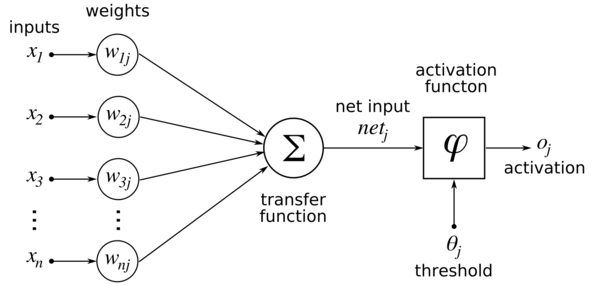
\includegraphics[width=0.8\textwidth]{images/nn_detail.png}
\caption{\label{fig:nnd} Shows the detailed working for one node in an artificial neural network.}
\end{figure}

\begin{figure}
\centering
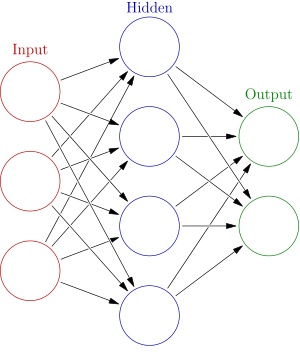
\includegraphics[width=0.4\textwidth]{images/nn_overview.png}
\caption{\label{fig:nno} Shows the general overview of an artificial neural network.}
\end{figure}